\documentclass{beamer}
\usepackage{ngerman}
\usetheme{Frankfurt}
\begin{document}
\title{ToureNPlaner}   
\author{Stupro Gruppe} 
\date{\today} 

\frame{\titlepage} 

\frame{\frametitle{"Ubersicht}\tableofcontents} 

\section{"Uber uns}
\subsection{Wer sind wir?} 
\frame{\frametitle{Wer sind wir?} 
ein "`freiwilliger"' Zusammenschluss aus 9 Studenten (8x Bsc. 5. Semester und 1x Diplom 7. Semester)
}
\subsection{Warum sind wir hier?}
\frame{ \frametitle{Warum sind wir hier?}
\begin{itemize}
\item Studienprojekt ist ein Pflichtmodul im Softwaretechnikstudium
\item Vollausgestatteter Arbeitsraum bietet mehr Ruhe als Arbeitsr"aume und Pools
\item ToureNPlaner hat auch noch eine Kaffeemaschine
\end{itemize}
}

\section{Studentenprojekt} 
\subsection{Was ist das Stupro?}
\frame{ \frametitle{Was ist das Stupro?}
\begin{itemize}
\item Projekt "uber 2 Semester
    \begin{itemize}
    \item 1 Semester projektspezifische Vorlesung besuchen
    \item 1 Seminar halten
    \item 1. und 2. Semester praktischer Teil (Softwareentwicklung)
    \end{itemize}
\item insgesamt 24 ECTS Punkte (720 Stunden)
\end{itemize}
}

\subsection{Was bringt das Stupro?} 
\frame{ \frametitle{Was bringt das Stupro?}
\begin{itemize}
\item {Praxiserfahrung Mit "`echten"' Kunden}
\item {Arbeiten in einem gro"sen Team}
\item {keine Micky Maus Programme}
\item {Programmiererfahrung}
\item {Softskills}
\end{itemize}
}


\subsection{Unser Projekt}
\frame{\frametitle{Unser Projekt}
ToureNPlaner soll folgende Aufgaben durchf"uhren:
\begin{itemize}

\item {Serveranwendung zur Routen- Tourenplanung realisieren}
\item {Zugriffsclients realisieren}
\begin{itemize}
\item {Webclient}
\item {Androidclient}
\end{itemize}
\end{itemize}

}
\section{Motivation}
\frame{\frametitle{Motivation}
\begin{itemize}
\item {Nicht triviale Routen \slash Tourenplanung berechnen}
\item {Postbote (DHL) will bestm"ogliche Rundtour finden}
\item {Fahrrad- und Elektroauto-Routen abh"angig von H"ohenmetern}
\end{itemize}
}

\section{Dijkstra Erkl"arung}
\frame{
Kartenansicht
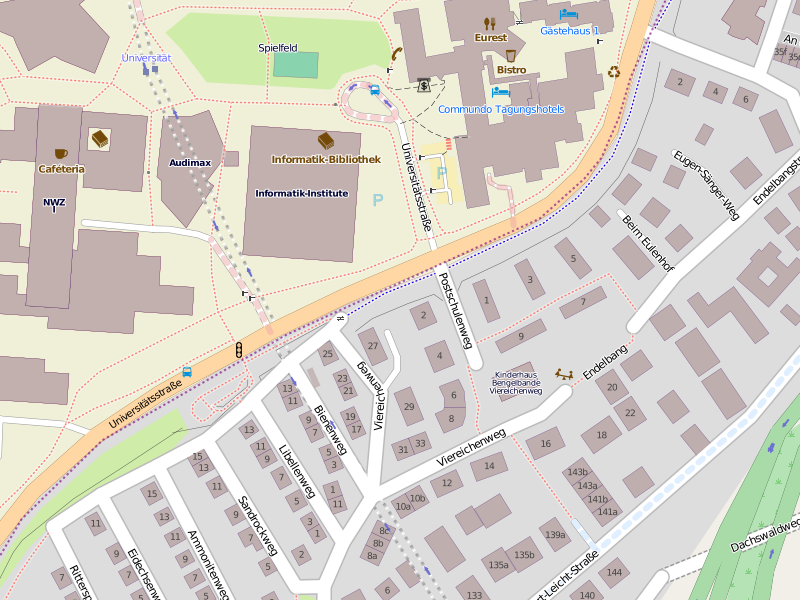
\includegraphics[width =\linewidth]{01.png}}
\frame{
Einf"ugen von Knoten
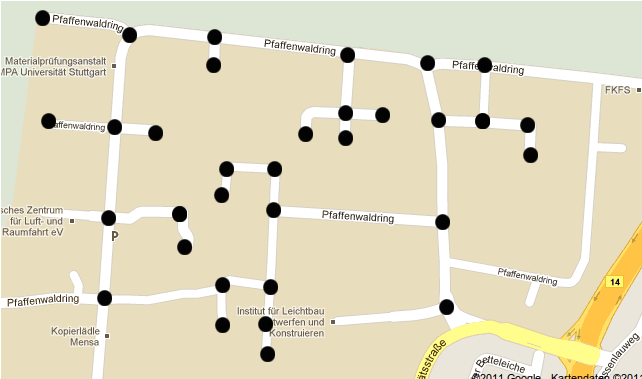
\includegraphics[width =\linewidth]{02.png}}
\frame{
Graphen erzeugen
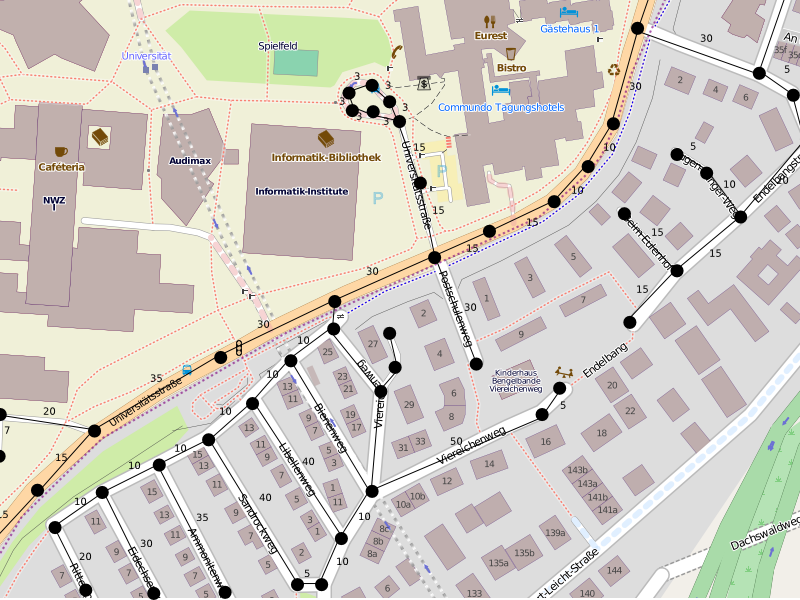
\includegraphics[width =\linewidth]{03.png}}
\frame{
Ziel und Startpunkt w"ahlen
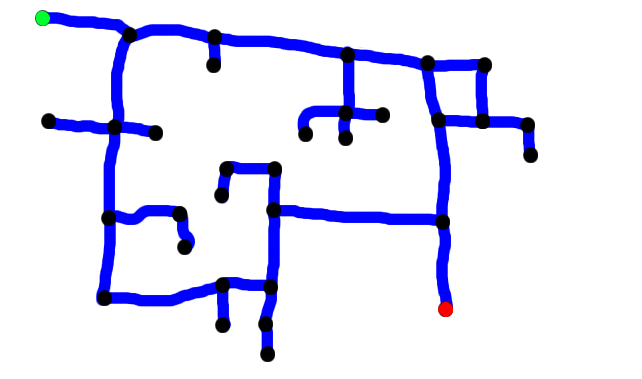
\includegraphics[width =\linewidth]{04.png}}
\frame{
K"urzesten Weg berechnen
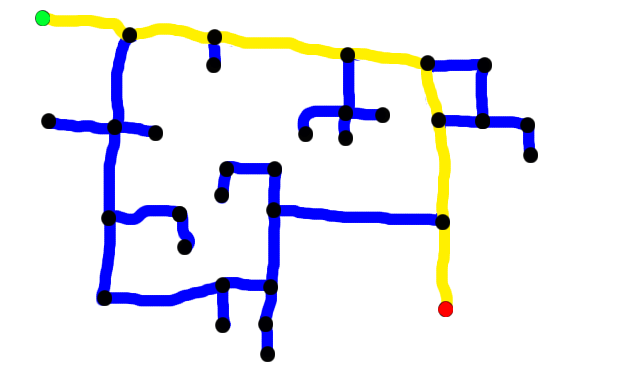
\includegraphics[width =\linewidth]{05.png}}

\section{LiveDemo}
\frame{\frametitle{LiveDemo}
\begin{itemize}
    \item Webclient
    \pause
    \item Android
\end{itemize}
}
\end{document}
